% !TEX root = ../main.tex
% NB: Denne filen bruker TikZ. Orkestrator: vennligst legg til
% \usepackage{tikz} i notes/preamble.tex hvis ikke allerede til stede.
\section{Salary vs.\ fringe benefits-modellen}\label{thr:salary-fringe-benefits-mix}

\paragraph{Definisjon.} Modellen for \emph{optimal mix mellom lønn (salary, $S$) og fringe benefits ($F$)} bestemmer hvordan bedriften skal sette sammen kompensasjonspakken slik at den ansattes \thref{reservation-utility}{reservation utility} oppfylles til lavest mulig kostnad for bedriften. Optimum oppstår der den ansattes \emph{indifferenskurve} er tangent til bedriftens \emph{isokostnadslinje}: bedriftens marginal-substitusjonsrate i kostnad er lik den ansattes marginal-substitusjonsrate i nytte. [SLIDE/BOK]

\subsection*{Forklaring}

Kompensasjon består typisk av (i) kontant lønn $S$ og (ii) fringe benefits $F$ -- pensjon, helseforsikring, firmabil, ekstra ferie, barnehageplass, lunsjordning, treningsmedlemskap, opsjoner med mer. Hvorfor ikke bare betale alt i lønn og la den ansatte velge selv?
\begin{enumerate}
\item \textbf{Skattefavør.} Mange fringe-elementer beskattes lavere enn lønn (pensjon, naturalytelser opp til grense). $1$ kr i fringe gir mer disponibel nytte enn $1$ kr i lønn $\Rightarrow$ bedriftens kostnad per nytte-enhet er lavere på $F$.
\item \textbf{Kvantumsrabatt / skala.} Bedriften får helseforsikring, abonnementer, kantine billigere per ansatt enn individet kan kjøpe alene.
\item \textbf{Superior assets.} Bedriften eier ressurser (kantine, kontorbygg, opplæringsprogram) som leverer nytte til ansatt til lav marginalkostnad -- jf.\ \thref{superior-assets}{superior assets}.
\item \textbf{Imperfekte substitutter.} Ansatte verdsetter $S$ og $F$ ulikt, og marginalmaten er fallende i hver komponent $\Rightarrow$ indifferenskurver er konvekse.
\end{enumerate}
[SLIDE]

\subsection*{Det formelle problemet}

Bedriften minimerer kostnaden $C(S,F) = c_S \cdot S + c_F \cdot F$ med bibetingelsen at den ansatte minst når reservation utility:
\[
  \min_{S,F} \; c_S \, S + c_F \, F \qquad \text{s.t.} \qquad U(S,F) \;\geq\; U_0 .
\]
Her er $c_S$ bedriftens marginalkostnad per krone lønn (typisk $> 1$ grunnet arbeidsgiveravgift, feriepenger, pensjon-på-pensjon), og $c_F$ er bedriftens marginalkostnad per nytte-enhet fringe. Hvis $c_F < c_S$ -- typisk pga.\ skatt eller skala -- gjøres det \emph{billigere} for bedriften å levere nytte via $F$ enn $S$. [BOK]

\paragraph{First-order condition.} I optimum gjelder
\[
  \mathrm{MRS}_{S,F} \;=\; \frac{\partial U / \partial S}{\partial U / \partial F} \;=\; \frac{c_S}{c_F}.
\]
Den ansattes vilje til å gi opp fringe for én ekstra krone lønn skal være lik bedriftens kostnadsforhold mellom de to. Geometrisk: tangering i $(S,F)$-planet mellom indifferenskurve $U_0$ og isokostnadslinje.

\subsection*{Modell / graf}

\begin{figure}[h]
  \centering
  
\includegraphics[width=0.35\linewidth]{BSZ_kap_14_2026/by_slide/slide_014/BSZ_kap_14_2026_slide_014_asset_01_image5.jpeg}
  \caption{Mengenrabatt: ``Mehr kaufen = mehr sparen'' -- kvantumsrabatter gjør fringe benefits billigere per enhet enn individuelt kjøp. (BSZ kap.\ 14, slide 14) [SLIDE]}
\end{figure}

\begin{figure}[h]
  \centering
  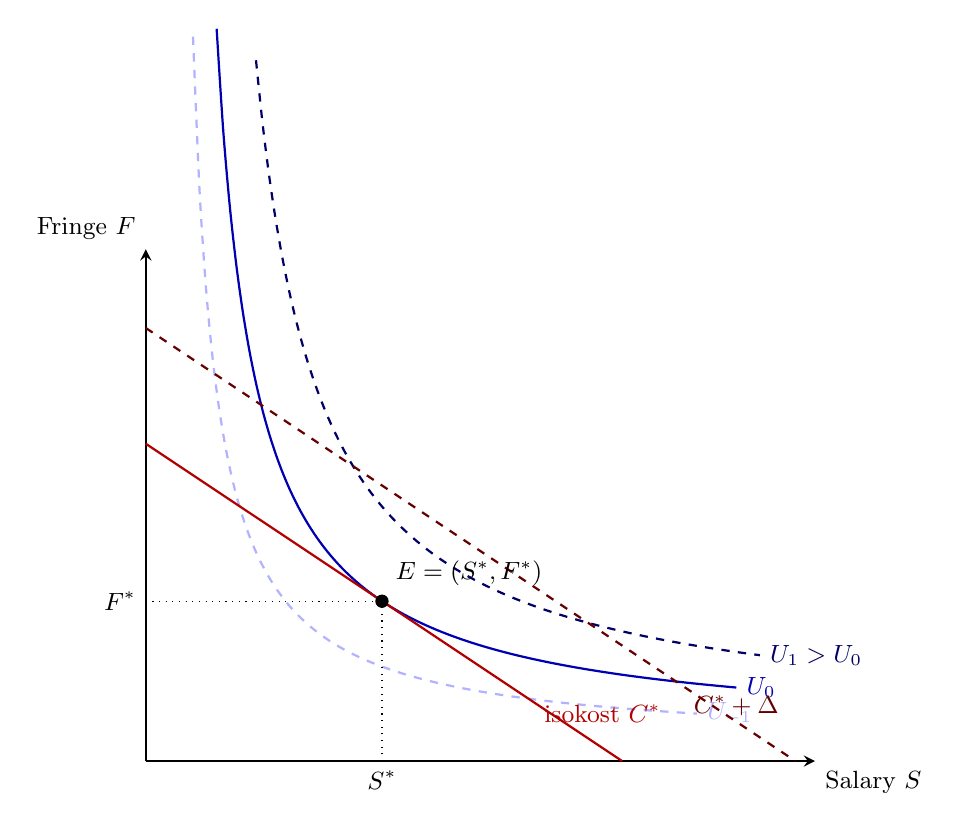
\begin{tikzpicture}[scale=1.0, >=stealth]
    % Akser
    \draw[->, thick] (0,0) -- (8.5,0) node[below right] {\small Salary $S$};
    \draw[->, thick] (0,0) -- (0,6.5) node[above left] {\small Fringe $F$};

    % Tre indifferenskurver (konvekse, U_0 nederst, så U_1, U_2)
    % U_0 -- reservation utility (passerer gjennom optimum)
    \draw[blue!70!black, thick, domain=0.9:7.5, smooth, samples=80]
      plot (\x, {4.5/(\x-0.4) + 0.3}) node[right] {\small $U_0$};
    % U_1 -- høyere nyttenivå
    \draw[blue!40!black, thick, dashed, domain=1.4:7.8, smooth, samples=80]
      plot (\x, {6.8/(\x-0.6) + 0.4}) node[right] {\small $U_1 > U_0$};
    % U_-1 -- lavere nyttenivå (under reservation -- ikke akseptert)
    \draw[blue!30, thick, dashed, domain=0.6:7.0, smooth, samples=80]
      plot (\x, {2.7/(\x-0.3) + 0.2}) node[right] {\small $U_{-1}$};

    % Isokostnadslinjer (rette, fallende). Helning = -c_S / c_F
    % Velg tangering i (3, 2)-ish. Helning = -1/2 (c_S=1, c_F=2 -- F billigere)
    % U_0 = 4.5/(x-0.4)+0.3 ; dU/dx = -4.5/(x-0.4)^2
    % I x=3: dy/dx = -4.5/(2.6)^2 = -4.5/6.76 = -0.666
    % => velg c_S/c_F = 0.666 => helning -0.666
    % Linje gjennom (3, 4.5/2.6+0.3) = (3, 2.03)
    % Linje: y = 2.03 - 0.666(x-3) -> x-skjær: 2.03/0.666 + 3 = 6.05
    %                                y-skjær: 2.03 + 0.666*3 = 4.03
    \draw[red!70!black, thick] (0, 4.03) -- (6.05, 0) node[below] {};
    \node[red!70!black] at (5.8, 0.6) {\small isokost $C^*$};

    % En høyere isokost (svakere)
    \draw[red!40!black, thick, dashed] (0, 5.5) -- (8.25, 0);
    \node[red!40!black] at (7.5, 0.7) {\small $C^* + \Delta$};

    % Optimum-punkt
    \filldraw[black] (3, 2.03) circle (2.2pt);
    \node[anchor=south west] at (3.05, 2.1) {\small $E = (S^*, F^*)$};

    % S* og F* akse-projiseringer
    \draw[dotted] (3, 0) -- (3, 2.03);
    \draw[dotted] (0, 2.03) -- (3, 2.03);
    \node[below] at (3, 0) {\small $S^*$};
    \node[left] at (0, 2.03) {\small $F^*$};
  \end{tikzpicture}
  \caption{Optimal mix mellom lønn ($S$) og fringe benefits ($F$). Den ansattes indifferenskurver $U_{-1}, U_0, U_1$ er konvekse mot origo (imperfekte substitutter). Bedriftens isokostnadslinjer har helning $-c_S / c_F$. I optimum $E$ tangerer reservation-utility-kurven $U_0$ den laveste oppnåelige isokostnadslinjen $C^*$: $\mathrm{MRS}_{S,F} = c_S/c_F$. Lavere kostnad ($C^* - \Delta$) når ikke $U_0$; høyere kostnad ($C^* + \Delta$) er sløsing. [SLIDE]}
\end{figure}

\paragraph{Hvordan grafen flyttes av endringer.}
\begin{itemize}
\item \textbf{Skatt på lønn øker} $\Rightarrow$ $c_S$ stiger $\Rightarrow$ isokostnadslinjen blir \emph{brattere} $\Rightarrow$ tangering flytter mot mer $F$, mindre $S$.
\item \textbf{Bedriften får kvantumsrabatt på forsikring} $\Rightarrow$ $c_F$ faller $\Rightarrow$ isokost blir flatere $\Rightarrow$ mer $F$ optimal.
\item \textbf{Reservation utility stiger} (stramt arbeidsmarked) $\Rightarrow$ $U_0$ flyttes utover $\Rightarrow$ minimumskostnaden $C^*$ stiger; mixen kan endre seg avhengig av preferanser.
\item \textbf{Heterogene ansatte} $\Rightarrow$ ulike indifferenskurver $\Rightarrow$ ulik optimal mix $\Rightarrow$ rasjonale for ``cafeteria-style benefits''.
\end{itemize}

\subsection*{Kjerneforutsetninger}
\begin{itemize}
\item $S$ og $F$ er \emph{imperfekte substitutter} i ansattes nytte -- begge har positiv, men avtakende marginalnytte.
\item Ansattes nyttefunksjon er kvasi-konkav (gir konvekse indifferenskurver).
\item Bedriftens kostnadsfunksjon er lineær eller konveks i $S$ og $F$.
\item $c_S \neq c_F$ -- ellers ville mix være likegyldig (kun totalbeløpet teller).
\item Bedriften kjenner -- eller estimerer rimelig -- ansattes preferanser.
\item Reservation utility $U_0$ er bindende.
\end{itemize}

\subsection*{Muligheter}
\begin{itemize}
\item Forklarer hvorfor lønn alene aldri er optimal kompensasjon når skatt og skala favoriserer fringe.
\item Begrunner cafeteria-style benefits og fleksibel kompensasjon for å håndtere preferanseheterogenitet.
\item Operasjonaliserer hvordan bedriften kan møte $U_0$ rimeligere -- direkte konkurransefordel.
\item Forklarer empirisk variasjon i lønnsmix på tvers av bedrifter, bransjer og land.
\item Gir formelt grunnlag for design av pensjons- og helseordninger.
\end{itemize}

\subsection*{Begrensninger og kritikk}
\begin{itemize}
\item \textbf{Heterogene preferanser.} Indifferenskurven varierer mellom ansatte; én pakke passer ikke alle (men cafeteria-løsninger reduserer problemet).
\item \textbf{Signaling-effekter.} Høy lønn kan signalere status og prestasje; å konvertere lønn til fringe kan rammes som ``lavere status'' selv om kontantverdien er den samme.
\item \textbf{Reference dependence.} Ansatte sammenligner lønn med kolleger; fringe er mindre synlig. For konkurransepress kan synlig lønn virke sterkere enn faktisk nytte tilsier.
\item \textbf{Likviditetspreferanse.} Unge ansatte med boliglån verdsetter kontantlønn (lav diskontering av fremtidig pensjon) mer enn modellen antar.
\item \textbf{Skatteregimer endres.} Et fringe-tungt design som er optimalt i dag kan bli suboptimalt etter politisk skift.
\item \textbf{Måleproblemer.} Verken $U(S,F)$ eller $c_F$ er presist kjent; tangering er konseptuell.
\item \textbf{Asymmetrisk informasjon.} Ansatte kjenner egne preferanser bedre enn bedriften $\Rightarrow$ \thref{adverse-selection}{adverse selection}: bedriften vet ikke hva den enkelte verdsetter.
\item \textbf{Insentiv-effekter på fringe.} Fringe gir typisk svakere prestasjonsinsentiv enn variabel lønn -- modellen ignorerer \thref{moral-hazard}{moral hazard}.
\end{itemize}

\subsection*{Eksempler}
\begin{itemize}
\item \textbf{Equinor.} Tung pensjonsordning, helseforsikring, lange ferieavtaler -- $c_F$ lav fordi statlig pensjonsstruktur og skala. Total mix har relativt høyt $F$-innslag og moderat $S$ relativt til amerikanske oljemajors. [EKS]
\item \textbf{Konsulent / investment banking (IBM, Goldman).} Lite fringe, høy bonus -- $c_F$ ikke spesielt fordelaktig, og ansatte er typisk mobile (lav verdi av pensjon hos én arbeidsgiver). Optimal mix tipper mot $S$ og kortsiktig bonus. [EKS]
\item \textbf{Novo Nordisk.} Omfattende familiefringe (helseforsikring, barnepass) hever pakkenytten for forskere som ofte har dual-career ektefelle og barn. Skattefavør i Danmark + skala. [EKS]
\item \textbf{Norsk offentlig sektor.} Lav $S$, men sterk pensjonsordning (Statens pensjonskasse) og jobbsikkerhet -- $F$-tung pakke som leverer høy $U_0$ til lav kostnad. [EKS]
\item \textbf{Cafeteria-plan i Mærsk.} Heterogene ansatte $\Rightarrow$ ansatte velger mellom ekstra ferie, pensjon, bilordning, ekstra helseforsikring; samme totalbudsjett, høyere nytte. [CASE]
\end{itemize}

\subsection*{Kobling til søyle og andre teorier}
Søyle: primært \SThree\ (insentivstruktur / kompensasjonsdesign). Modellen tar \thref{reservation-utility}{reservation utility} som bibetingelse, justerer for \thref{compensating-differentials}{compensating differentials} (uattraktive trekk hever $U_0$), og utnytter \thref{superior-assets}{superior assets} (lav $c_F$ via skala/kultur/skatt). Knyttet til \thref{principal-agent}{prinsipal--agent} (participation constraint), \thref{specific-vs-general-knowledge}{spesifik humankapital} (firm-spesifik fringe binder ansatt) og \thref{moral-hazard}{moral hazard} (fringe vs.\ variabel lønn-trade-off).

\paragraph{Brukt i spørsmål:} Q08.
